\section{Design Decisions}
\label{netqasm:sec:design_decisions}

Based on the use-cases, design considerations and requirements, we have designed the low-level language \ac{NetQASM} as an API to the \ac{QNPU}.
In this section we present concepts and design decisions we have taken.
Details on the mode of execution and the \ac{NetQASM}-language are presented in \cref{netqasm:sec:implementation}.

\subsection{Interface between \ac{CNPU} and QNPU}
\label{netqasm:sec:design_decisions_interface}

\subsubsection{Execution model}
As described in \cref{netqasm:sec:abstract_model}, and also in \cref{netqasm:sec:design_considerations} program execution is split across the \ac{CNPU} and the \ac{QNPU}.
Since the \ac{QNPU} is assumed to have limited processing power (\cref{netqasm:sec:abstract_model}), our design lets the \ac{CNPU} do most of the classical processing.
The program blocks (\cref{netqasm:fig:program_decomp}) are hence spread over two separate systems: blocks of purely classical code are executed by the \ac{CNPU}, and blocks of quantum code (containing both quantum operations and limited classical control) are executed by the \ac{QNPU}.

The quantum code (including limited classical control) is expressed using the \ac{NetQASM} language.
The classical code is handled completely by the \ac{CNPU}, and we do not impose a restriction to its format.
In our implementation (\cref{netqasm:sec:python-sdk}), we use Python.
This classical code on the \ac{CNPU} also handles all application-level classical communication between nodes, since it cannot be done on the \ac{QNPU}.

We let the \ac{CNPU} initiate a program.
Whenever quantum code needs to be executed, the \ac{CNPU} delegates this to the \ac{QNPU}.
Since processing delay should be minimized (\cref{netqasm:sec:design_considerations}), the communication between \ac{CNPU} and \ac{QNPU} should be minimized.
Therefore, \ac{NetQASM} bundles the quantum operations together into blocks of instructions, called \textit{subroutines}, to be executed on the \ac{QNPU}.
A program, then, consists of both both classical code and quantum code, and the quantum code is represented as one or more subroutines.
These subroutines can be seen as the quantum code blocks of~\cref{netqasm:fig:program_decomp}.

For most programs, we consider subroutines to be sent consecutively in time.
However, if the \ac{QNPU} supports it, \ac{NetQASM} also allows to send multiple subroutines to be executed on the \ac{QNPU} at the same time, although this requires some extra care when dealing with shared memory.
From the perspective of the \ac{QNPU}, a program consists of a series of subroutines sent from the \ac{CNPU}.
Before receiving subroutines, the \ac{CNPU} first \textit{registers} a program at the \ac{QNPU}.
The \ac{QNPU} then sets up the classical and quantum memories (see below) for this program.
Then, the \ac{CNPU} may send subroutines to the \ac{QNPU} for execution.


\subsubsection{Shared classical memory}
Since classical and quantum blocks in the code (as per \cref{netqasm:fig:program_decomp}) can depend on each other, the \ac{CNPU} and the \ac{QNPU} need to have a way to communicate information to each other.
For example, a subroutine may include a measurement instruction; the outcome of this measurement may be used by the \ac{CNPU} upon completion of the subroutine.
Therefore, \ac{NetQASM} uses a shared memory model such that conceptually both layers can access and manipulate the same data. This solves the need to return data, and to do conditionals (\cref{netqasm:sec:design_considerations}).

Each program has a classical memory space consisting of \textit{registers} and \textit{arrays}.
Registers are the default way of storing classical values, like a measurement outcome.
In the example of the \ac{CNPU} needing a measurement outcome, there would be an instruction in the subroutine saying that a measurement outcome needs to be placed in a certain register.
The \ac{CNPU} can then access this same register (since they share the memory space) and use it in further processing.
The number of registers is small, and constant for each program.
Arrays are collections of memory slots (typically the slots are contiguous), which can be allocated by the program at runtime.
Arrays are used to store larger chunks of data, such as parameters for entanglement requests, entanglement generation results, or multiple measurement outcomes when doing multiple entangle-and-measure operations.
The \ac{CNPU} may only read from the shared memory; writing to it can only be done by issuing \ac{NetQASM} instructions such as \texttt{set} (for registers) and \texttt{store} (for arrays).
The \ac{QNPU} may directly write to the shared memory, for example when entanglement finished and it writes the results to the array specified by the program.


\begin{figure}[t]
      \centering
      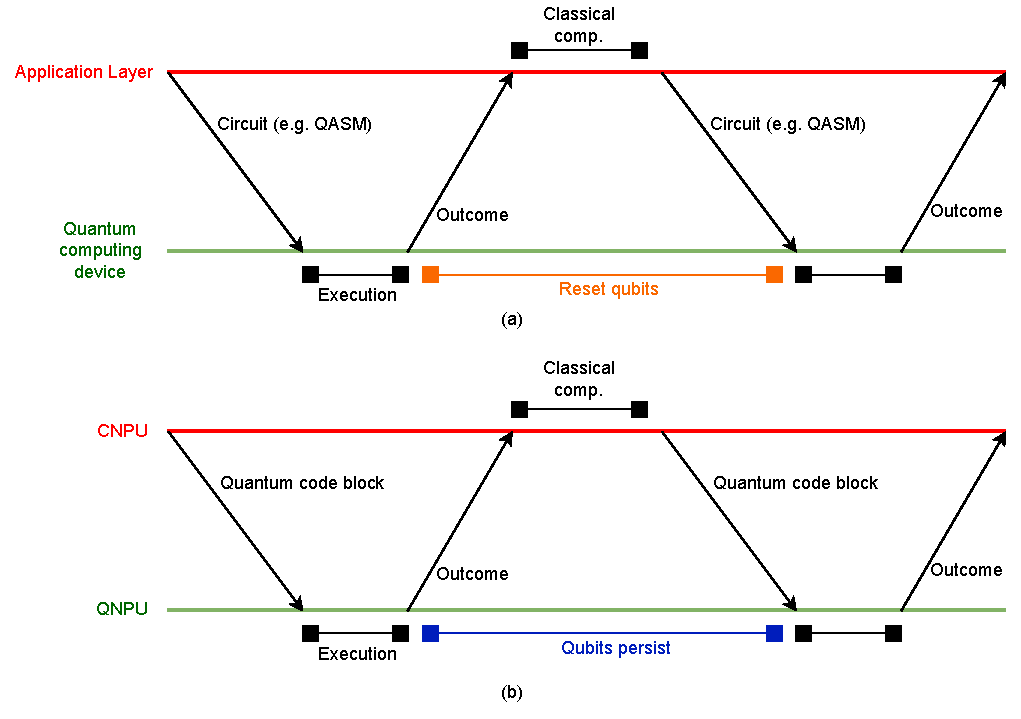
\includegraphics[width=0.8\linewidth]{figures/netqasm/classical-quantum-interaction.pdf}
      \caption{Program interaction between the \ac{CNPU} and a quantum device in
            both the case of \emph{hybrid-quantum computing} (a)
            and quantum networks (b). In the case of hybrid-quantum
            computing, qubits are reset in between circuits (in e.g. QASM). For
            quantum internet programs the qubits should on the other hand be
            kept in memory, since they might be entangled with another node and
            intended to be used further.}
      \label{netqasm:fig:hybrid}
\end{figure}

\subsubsection{Unit modules}
In order to support systems with multitasking (\cref{netqasm:sec:design_considerations}), \ac{NetQASM} provides a virtualized model of the quantum memory to the program.
This allows the \ac{QNPU} to do mapping between the virtualized memory and the physical memory and perform scheduling between programs.

The quantum memory for a program is represented by a \textit{unit module} (\cref{netqasm:fig:topology}).
A unit module defines the topology of the available qubits (which qubits are connected, i.e. on which qubit pairs a two-qubit gate can be executed), plus additional information on each qubit.
This additional information consists of which gates are possible on which qubit or qubit pair.
It also specifies if a qubit can be used for remote entanglement generation or not.
The extra information is needed since on some platforms, not all qubits can be used for entanglement generation and different qubits may support different local gates.
For example, in a single NV-centre, there is only one communication qubit and any additional qubits are storage qubits.
Also, the communication qubit can do different local gates than the storage qubits.

A single program has a single quantum memory space, which is \textit{not} reset at the end of a subroutine, which is in contrast with quantum computing.
This allows the \ac{CNPU} to do processing while qubits are in memory.
The following sequence of operations provides an example.
    (1) The \ac{CNPU} first sends a subroutine containing instructions for entanglement generation with a remote node R.
    (2) The \ac{QNPU} has finished executing the subroutine, and informs the \ac{CNPU} about it.
        There is now a qubit in the program's memory that is entangled with some qubit in R.
    (3) The \ac{CNPU} does some classical processing and waits for a classical message from (the \ac{CNPU} of) R.
    (4) Based on the contents of the message, the \ac{CNPU} sends a new subroutine to the \ac{QNPU} containing instructions to do certain operations on the entangled qubit.
        The subroutine can indeed access this qubit by using the same identifier as the first subroutine, since the quantum memory is still the same.
        We note the contrast with (non-network) quantum computing, where quantum memory is reset at the end of each block of instructions (\cref{netqasm:fig:hybrid}).


Unit modules contain \textit{virtual qubit IDs}.
This is because of the requirement that it should be possible to run multiple programs at the same time on a single \ac{QNPU} (Multitasking consideration in \cref{netqasm:sec:design_considerations}).
We use an approach that is similar to virtual memory in classical systems~\cite{arpaci2018operating}.
Each application has control over a set of physical qubits, but the application does not (need to) know which physical qubits these are exactly.
The unit module provides a virtualized view of this available memory.
This view contains virtual IDs each representing a single qubit, called a virtual qubit.
The \ac{QNPU} maintains a mapping of virtual IDs (per application) to physical qubits.
The \ac{QNPU} may change this mapping over time, without the applications knowing.
We stress that our virtualization hence only involves a mapping from IDs to physical qubits.
There is no copying of quantum states involved.

We note that this design decision meets our Multitasking consideration(\cref{netqasm:sec:design_considerations}).
By using virtualized unit modules, the \ac{QNPU} is free to map qubit IDs of the application to physical qubits as it sees fit.
For example, consider a node with a physical memory consisting of one communication qubit, and multiple memory qubits.
Application A creates entanglement with a remote node such that its half of the pair is in the communication qubit.
Then, application A needs to wait for a long time before further processing the quantum state in this qubit, for example since it needs to wait for a classical message from a remote node.
Meanwhile, application B is waiting to be executed on the \ac{QNPU}, and it also requires the communication qubit for entanglement generation.
The \ac{QNPU} can now move the state from the communication qubit to one of the memory qubits, and update the mapping of application A's ID to this physical memory qubit.
Then, the \ac{QNPU} can run application B while A is waiting for the classical message.
When B has finished, the \ac{QNPU} can move A's state back to the communication qubit.
Since application A uses the unit module and does not know about the physical memory, it
    (1) does not care that its state was temporarily moved to a different physical qubit, and
    (2) can remain oblivious about any other application being run (like B) while it is waiting.


\begin{figure}[t]
      \centering
      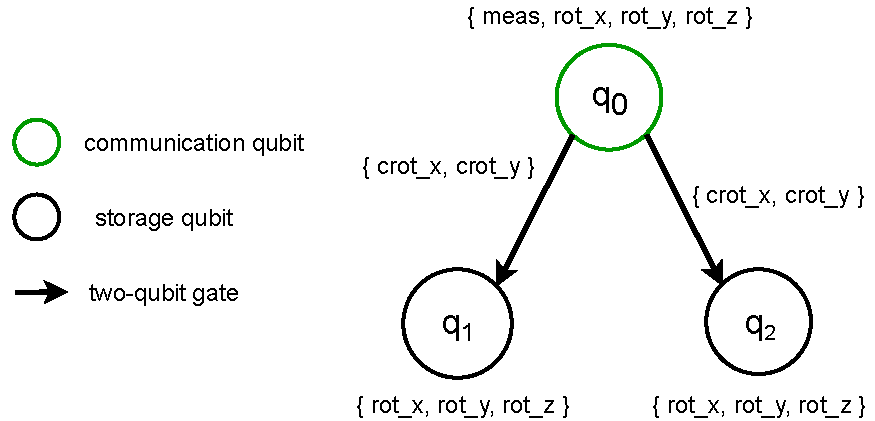
\includegraphics[width=0.6\linewidth]{figures/netqasm/unit-module.pdf}
      \caption{Example of a unit-module topology on a platform using
            nitrogen-vacancy centers in diamond. A unit-module is a
            hypergraph~\cite{berge1984hypergraphs}, with associated information
            on both nodes and edges. Each node represents a virtual qubit,
            containing information about (1) its qubit type (communication or
            storage), (2) physical properties of the qubit, such as decoherence
            times and (3) which single-qubit gates are supported on the qubit,
            together with their duration and noise. Each edge represents the
            possibility of performing joint operations on those qubits, such as
            two-qubit gates, and also containing information about gate
            durations and noise.}
      \label{netqasm:fig:topology}
\end{figure}



\subsection{NetQASM language}

\subsubsection{Instructions}
\label{netqasm:sec:design_decisions_language}
As explained in~\cref{netqasm:sec:design_decisions_interface}, the \ac{CNPU} delegates quantum code (including limited classical control) of the program to the \ac{QNPU} by creating blocks of instructions and sending these to the \ac{QNPU} for execution.
These blocks are called subroutines and contain \ac{NetQASM} \textit{instructions}.
Since the \ac{QNPU} is meant to be limited in processing power, the instruction set that it interprets should also be simple and low-level.
The \ac{NetQASM} instruction set contains instructions for simple arithmetic, classical data manipulation, and simple control flow in the form of (un)conditional branch instructions.
Although conditional control-flow can be done at the \ac{CNPU} as well, \ac{NetQASM} branching instructions allow for much faster feedback since they are executed by the \ac{QNPU}, and hence cover the design consideration of real-time conditionals (\cref{netqasm:sec:design_considerations}).
We note the obvious performance gain by being able to do control logic without having to go back to the \ac{CNPU}.
There are no higher-level concepts such as functions or for-loops, which would require more complicated and resource-demanding parsing for the \ac{QNPU}, such as constructing an abstract syntax tree.

A single instruction specifies an operation, possibly acting on classical or quantum data.
For example, a single-qubit rotation gate is represented as an instruction containing the type of gate, the classical register containing the rotation angle, and the classical register containing the virtual ID of the qubit (as specified in the unit module) to act on.
\ac{NetQASM} specifies a set of \textit{core} instructions that are expected to be implemented by any \ac{QNPU}.
These include classical instructions like storing and loading classical data, branching, and simple arithmetic.
Different hardware platforms support different quantum operations.
\ac{NetQASM} should also support platform-specific optimization (\cref{netqasm:sec:design_considerations}).
Therefore, \ac{NetQASM} uses \textit{flavors} of quantum instructions (\cref{netqasm:sec:design_decisions_flavours}).
The \textit{vanilla} flavor consists universal of a set of platform-independent quantum gates.
Particular hardware platforms, such as the NV-centre, may use a special NV flavor, containing NV-specific instructions.
A \ac{QNPU} implementation may use a custom mapping from vanilla instructions to platform-specific ones.
The instructions in a flavor are also called a software-visible gate set~\cite{murali2019fullstack}.
See~\cref{netqasm:sec:instructions} for more details on \ac{NetQASM} instructions.

\subsubsection{Remote entanglement generation}
Generating entanglement with a remote node is also specified by instructions.
These are however somewhat special compared to other instructions.
First, entanglement generation has a non-deterministic duration.
Therefore, when an entanglement instruction is executed, the request is forwarded to the part of the system responsible for creating entanglement, but the instruction itself immediately returns.
A separate \textit{wait} instruction can be used to block on entanglement generation to actually be completed.
Second, entanglement generation requests should be compatible with the network stack proposed in~\cite{dahlberg2019linklayer}, including the network layer from~\cite{kozlowski2020networklayer}.
These requests need to be accompanied by information such as the number of EPR pairs to generate or the minimum required fidelity.
Third, this information should be able to depend on runtime information.
For example, the required fidelity may depend on an earlier measurement outcome.
Therefore, entanglement generation parameters cannot be static data, and must be stored in arrays.
Furthermore, the result of entanglement generation with the remote node consists of a lot of information, such as which Bell state was produced, the time it took, and the measurement results in case of measuring directly.
This information is written by the \ac{QNPU} to an array which is specified by the entanglement instruction.
Finally, since writing the information to the array indicates that entanglement generation succeeded, the wait instruction can be used to wait until a certain array is filled in, such as the one provided by the entanglement instruction.
Since the entanglement instruction is non-blocking, it is possible to continue doing local operations while waiting for entanglement generation to complete.

We assume that the \ac{QNPU} implements a network stack where connections need to be set-up between remote nodes before entanglement generation can happen~\cite{kozlowski2020networklayer, dahlberg2019linklayer}.
\ac{NetQASM} provides a way for programs to open such connections in the form of \textit{EPR sockets}.
The \ac{CNPU} can ask the \ac{QNPU} to open an EPR socket with a particular remote node.
The \ac{QNPU} is expected to set up the required connections in the network stack, and associates this program socket with the connection.
When the program issues an instruction for generating entanglement, it refers to the EPR socket it wants to use.
Based on this, the \ac{QNPU} can use the corresponding connection in the network.


\begin{figure}[t]
      \centering
      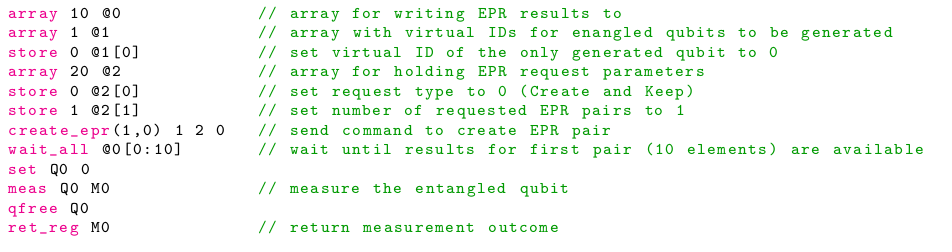
\includegraphics[width=0.6\linewidth]{figures/netqasm/nqasm_code_example}
      \caption{Example of NetQASM code for generating a single entangled pair with another node followed by a measurement.
            See the Appendix for more details of the instructions.}
      \label{netqasm:fig:nqasm_code_example}
\end{figure}

\subsubsection{Flavors}
\label{netqasm:sec:design_decisions_flavours}
We want to keep \ac{NetQASM} platform-independent.
However, we also want the potential for platform-specific optimization (\cref{netqasm:sec:design_considerations}).
Therefore we introduce the concept of \textit{flavors}.
Flavors only affect the quantum instruction set of the language, and not the memory model or the interaction with the \ac{QNPU}.
We use the \textit{vanilla} or generic flavor for a general, universal gate set.
Subroutines may be written or generated in this vanilla flavor.
Platform-independent optimization may be done on this level.
A \ac{QNPU} may directly support executing vanilla-flavored \ac{NetQASM}.
Platform-specific translations may then be done by the \ac{QNPU} itself.
It can also be that a \ac{QNPU} only supports a specific flavor of \ac{NetQASM}.
A reason for this could be that the \ac{QNPU} does not want to spend time translating of the instructions at runtime.
In this case, the \ac{CNPU} should perform a translation step from the vanilla flavor to the platform-specific flavor.
In such a case, the vanilla flavor can be seen as an \textit{intermediate representation}, and the translation to a specific flavor as a back-end compilation step.

\subsubsection{Programmability}
Since the \ac{NetQASM} instructions are relatively low-level, we like to have a higher-level programming language for writing programs, that is automatically compiled to \ac{NetQASM}.
We introduce a higher-level SDK in \cref{netqasm:sec:python-sdk}.
However, we do not see this as part of the \ac{NetQASM} specification itself.
This decoupling allows the development of SDKs to be independent such that these can be provided in various languages and frameworks.

We still want \ac{NetQASM} instructions to be suitable for manual writing and inspection.
Therefore, instructions (and subroutines) have two formats: a binary one that is used when sending to the \ac{QNPU}, and a text format that is human-readable.
The text format resembles assembly languages including OpenQASM.
Examples are given in \cref{netqasm:sec:python-sdk} and the Appendix.